\documentclass[10pt,twocolumn,a4paper]{article}
\usepackage[margin=0.7in,columnsep=0.25in]{geometry}
\usepackage{graphicx,amsmath,booktabs,caption,hyperref}
\captionsetup{font=small,skip=2pt}
\setlength{\parskip}{2pt}
\title{\vspace{-1.5cm}\textbf{RL-Based Smart Streetlight Control with Tabular Q-Learning}\vspace{-0.3cm}}
\author{\small TEAM MEMBERS: \textit{<names and roll numbers>}\\
\small GitHub: \url{https://github.com/Rohan1729-ju/rl-smart-streetlight}}
\date{\vspace{-0.6cm}AI Assignment 2 -- Real-Life Use Cases of RL}
\begin{document}
\maketitle
\vspace{-0.4cm}

\section{Problem}
Streetlights usually run at fixed brightness all night (or all day, with faulty photocells), wasting electricity when roads are empty or already bright. We cast brightness control as a Markov Decision Process in which an agent dims or brightens a lamp every 10 minutes to cut energy use while keeping the road adequately lit when pedestrians are present.

\section{RL Formulation}
\textbf{State space $S$.} The observation is discretised into
(time-of-day block $\in\{0..5\}$, 4 h each) $\times$ (ambient-light bin $\in\{0..3\}$, thresholds 10/30/60 units) $\times$ (pedestrian bin $\in\{0,1\text{--}2,3+\}$) $\times$ (previous brightness level $\in\{0..4\}$), giving $|S|=6\cdot4\cdot3\cdot5=360$ states. Previous brightness makes the flicker penalty Markovian.

\textbf{Action space $A$.} Five discrete dimming levels $b\in\{0,0.25,0.5,0.75,1\}$ of a 100\,W lamp (60 light units at full output).

\textbf{Reward $R$.} With ambient light $L_a$, required light $L_{req}$ (20 units on an empty road, 50 if pedestrians are present) and $n$ pedestrians,
\begin{equation}
\begin{split}
r_t = &-\alpha\, b_t \;-\; \beta\, \underbrace{\frac{\max(0,L_{req}-L_a-60\,b_t)}{L_{req}}}_{\text{shortfall}}\,\bigl(1+0.5\min(n,4)\bigr)\\
&-\gamma\,|b_t-b_{t-1}|,
\end{split}
\end{equation}
with $\alpha=1,\ \beta=3,\ \gamma=0.1$. The first term penalises electricity, the second penalises under-lighting (more heavily when more people are present), and the third discourages flickering.

\section{Environment and Algorithm}
\textbf{Simulator} (custom, NumPy only). One episode is a 24 h day of 144 steps. Ambient light follows a clipped sinusoid between 06:00 and 18:00 scaled by a per-day cloud factor $\sim U(0.4,1)$ plus Gaussian noise. Pedestrian counts are Poisson with a time-varying rate with morning (08:00), midday and evening (19:30) peaks and a near-zero night floor. Actions do not affect weather or pedestrians, so every policy can be evaluated on identical days.

\textbf{Algorithm.} Tabular Q-learning,
$Q(s,a)\!\leftarrow\!Q(s,a)+\eta\,[r+\delta\max_{a'}Q(s',a')-Q(s,a)]$, with $\eta=0.1$, $\delta=0.95$, $\epsilon$-greedy exploration decaying from 1.0 to 0.02 ($\times0.999$/episode), 6000 training episodes. Because all rewards are $\le0$, a zero-initialised table is optimistic and encourages exploration.

\textbf{Baselines.} Fixed 100\%, fixed 50\%, uniformly random, and a dusk-to-dawn photocell rule (100\% when ambient bin $\le1$, else off). All are evaluated with the greedy Q-policy on 500 unseen days.

\section{Results}
\begin{figure}[h]\centering
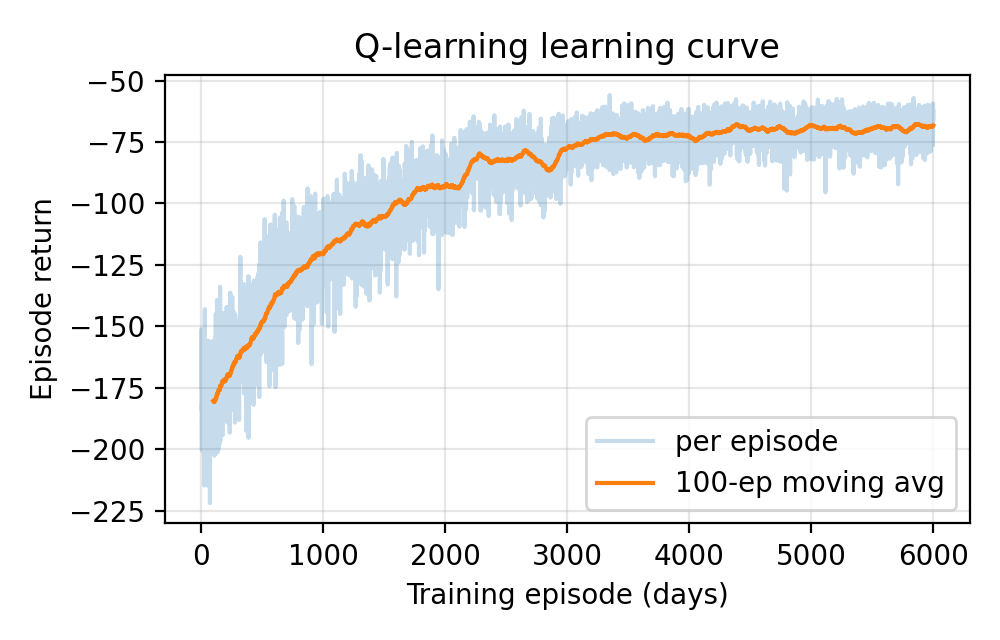
\includegraphics[width=\linewidth]{../results/learning_curve.png}
\caption{Learning curve: episode return improves from about $-180$ to $-69$ and plateaus after $\sim$4000 episodes.}
\end{figure}

\begin{table}[h]\centering\small
\begin{tabular}{lrrrr}\toprule
Policy & kWh/day & Return & Ped.\ unsafe\% \\\midrule
Fixed 100\% & 2.40 & $-144.1$ & 0.00 \\
Fixed 50\% & 1.20 & $-129.2$ & 50.66 \\
Random & 1.20 & $-186.8$ & 37.58 \\
Dusk-to-dawn & 1.57 & $-103.5$ & 8.21 \\
\textbf{Q-learning} & \textbf{1.03} & $\mathbf{-65.6}$ & \textbf{0.08} \\\bottomrule
\end{tabular}
\caption{Mean over 500 unseen days. ``Ped.\ unsafe'' = share of pedestrian-present steps with $>$20\% light shortfall.}
\end{table}

The agent uses \textbf{57\% less energy} than fixed 100\% brightness (1.03 vs.\ 2.40 kWh/day) with only 0.08\% under-lit pedestrian steps, and beats the dusk-to-dawn rule on both energy (34\% lower) and safety. Fixed 50\% saves energy but leaves half of pedestrian steps under-lit. Fig.~2 shows the learned policy: off in daylight, about 50\% on dark empty roads, and 75--100\% when pedestrians are present in the dark. A limitation is flicker: the agent changes level more often (total brightness change 18.5 per day vs.\ $\le1$) than fixed policies; raising $\gamma$ would trade energy for smoothness.

\begin{figure}[h]\centering
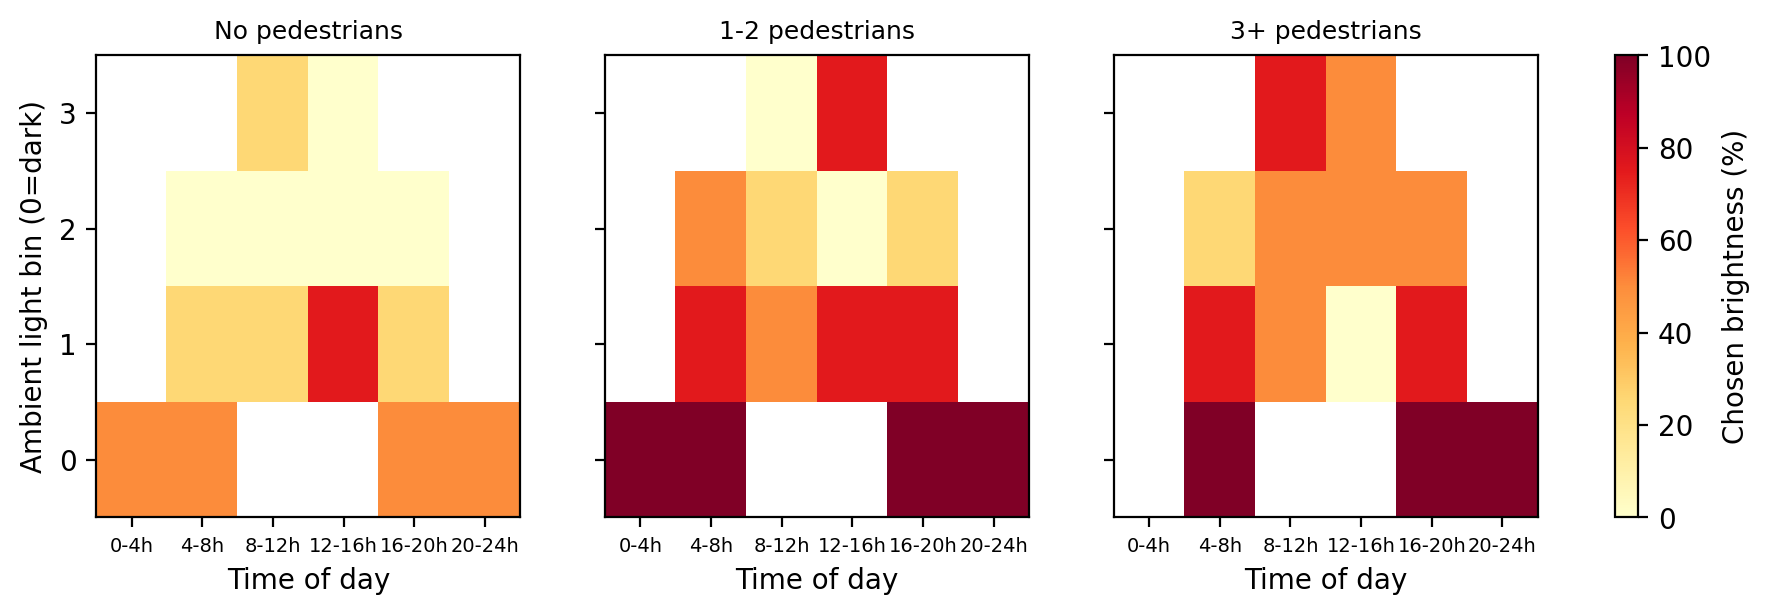
\includegraphics[width=\linewidth]{../results/policy_heatmap.png}
\caption{Greedy brightness by time block and ambient bin (previous level 50\%). Blank cells are unvisited states.}
\end{figure}

\textbf{Sensitivity.} Sweeping $\beta\in\{0.5,\dots,10\}$ (Fig.~3) traces an energy--safety frontier: low $\beta$ saves energy (0.46 kWh/day) but leaves 51\% of pedestrian steps under-lit, while $\beta\ge2$ reaches near-zero violations at about 1.0--1.1 kWh/day.

\begin{figure}[h]\centering
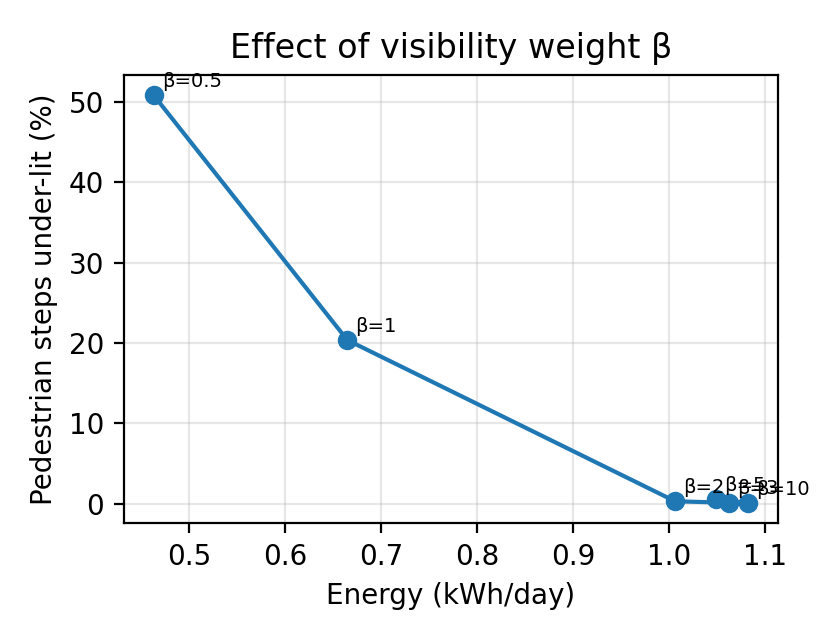
\includegraphics[width=0.8\linewidth]{../results/sensitivity_beta.png}
\caption{Effect of the visibility weight $\beta$ on energy and safety.}
\end{figure}

\section{Conclusion}
A tabular Q-learning agent learns an interpretable dimming policy that substantially reduces energy while maintaining pedestrian visibility. Future work: multiple coordinated lamps, function approximation (DQN) for continuous states, and real sensor data.

\end{document}
